%*******************************************************************************
% Definicje stylu dokumentu
%*******************************************************************************

%===============================================================================
% klasa dokumentu

%\documentclass[12pt, a4paper, twoside, titlepage, final]{mwbk}
%\documentclass[10pt,a4paper,onecolumn,oneside,11pt,wide,floatssmall]{book}
\documentclass[10pt,a4paper]{article}


%===============================================================================
% Pakiety
%\usepackage[latin2]{inputenc}
\usepackage{polski}
%\usepackage[cp1250]{inputenc}
\usepackage[utf8]{inputenc}				% kodowanie �r�d�a
\usepackage[polish]{babel}				% polskie przenoszenie wyraz�w (hyph.)
\usepackage[T1]{fontenc}					% font PL
\usepackage{url}								% polecenie \url
\usepackage{amsfonts}						% fonty matematyczne
\usepackage{graphicx}						% wstawianie grafiki
\usepackage{color}							% kolory
\usepackage{fancyhdr}						% paginy g�rne i dolne
\usepackage[plainpages=false]{hyperref}		% dynamiczne linki
\usepackage{calc}							% operacje arytmetyczne w TeX'u
\usepackage{tabularx}						% rozci�gliwe tabele
\usepackage{array}							% standardowe tabele
\usepackage{geometry}
\usepackage{hyperref}
\usepackage{subfigure}
\usepackage{wrapfig}
\usepackage{indentfirst}
\usepackage{amsmath}
\usepackage{color}
\usepackage{array}
\usepackage{pdflscape}
\usepackage{amsmath}
\usepackage{textcomp}
\usepackage[font={small,it}]{caption}
\usepackage{etoolbox}
\usepackage[section]{placeins}
\usepackage{float}


% \linespread{1.3}								% 1.3 do interlinii 1.5


% \patchcmd{\thebibliography}{\chapter*}{\section*}{}{}

% \bibliographystyle{plain}
% % w�asne pakiety

% %===============================================================================
% % Ustawienia dokumentu

% \frenchspacing

% % ustawienia wymiar�w
% \oddsidemargin 0mm							% margines nieparzystych stron
% \evensidemargin 0mm							% margines parzystych stron
% \headheight 15pt								% wysoko�� paginy g�rnej
% \topmargin 0mm									% margines g�rny
% \setlength{\parindent}{0pt}
% \setlength{\parskip}{1ex plus 0.5ex minus 0.2ex}
% styl paginacji
 \pagestyle{fancy}
% % \renewcommand{\chaptermark}[1]{}%{\markboth{#1}{}} % BO ARTICLE
% \renewcommand{\sectionmark}[1]{}%{\markright{\thesection\ #1}{}}
% \renewcommand{\thesection}{\arabic{section}}


 % naglowek 
 \fancyhf{}
 \fancyhead[R]{\thepage}
 \fancyhead[L]{[BD2]~System wspierający pracę szpitala - faza logiczna}
% %\fancyhead[LO]{\small\nouppercase{\rightmark}}
% %\fancyhead[R]{\small\nouppercase{\leftmark}}
\renewcommand{\headrulewidth}{0.1pt}
\renewcommand{\footrulewidth}{0pt}

% % nag��wek w stylu plain 
\fancypagestyle{plain}
{
\fancyhf{}
\renewcommand{\headrulewidth}{0pt}
\renewcommand{\footrulewidth}{0pt}
}

% % ta sekwencja tworzy czyste kartki na stronach po \cleardoublepage
% \makeatletter
% \def\cleardoublepage{\clearpage\if@twoside \ifodd\c@page\else
% 	\hbox{}
% 	\vspace*{\fill}
% 	\thispagestyle{empty}
% 	\newpage
% 	\if@twocolumn\hbox{}\newpage\fi\fi\fi}
% \makeatother

% %===============================================================================
% % Zmienne �rodowiskowe i polecenia

% % definicja
% % \newtheorem{definition}{Definicja}[chapter] % BO CHAPTER
% \newtheorem{definition}{Definicja}

% % twierdzenie
% % \newtheorem{theorem}{Twierdzenie}[chapter] % BO CHAPTER
% \newtheorem{theorem}{Twierdzenie}

% % obcoj�zyczne nazwy
% \newcommand{\foreign}[1]{\emph{#1}}

% % pozioma linia
% \newcommand{\horline}{\noindent\rule{\textwidth}{0.4mm}}

% % wstawianie obrazk�w {plik}{caption}{opis}
% \newcommand{\fig}[3]
% {
% \begin{figure}[!htb]
% \begin{center}
% \includegraphics[width=\textwidth]{#1}
% \caption[#2]{#2. #3}
% \label{#1}
% \end{center}
% \end{figure}
% }

% %===============================================================================
% % ustawienia pakietu hyperref

% \hypersetup
% {
% %colorlinks=true,			% false: boxed links; true: colored links
% %linkcolor=black,			% color of internal links
% %citecolor=black,			% color of links to bibliography
% %filecolor=black,			% color of file links
% %urlcolor=black			% color of external links
% }

% %===============================================================================

\title{Bazy Danych 2 \\ \Huge{System wspierający pracę szpitala} \\ \Large{Dokumentacja projektu - faza logiczna} }
\author{ Piotr Małetka \\ Radosław Świątkiewicz \\ Marek Majde \\ Michał Dobrzański \\ \\ Politechnika Warszawska, \\ Wydział Elektroniki i Technik Informacyjnych.}

\begin{document}
\maketitle

\newpage

\section{Błędy fazy konceptualnej}
Formatowanie dokumentacji z fazy pierwszej zostało gruntownie poprawione;
kolejne fazy dokumentacji będą tworzone w środowisku \LaTeX , aby zapewnić przejrzystość dokumentacji oraz spójność formatowania.

\textbf{Poprawiono diagram encji} tak, aby stał się bardziej czytelny.
Zwiększono odległości między encjami, linie symbolizujące związki nie nachodzą na siebie; nie są przesłaniane przez inne encje.
Diagram jest obrazem o wysokiej rozdzielczości umożliwiającej na znaczne powiększenie schematu.


\textbf{Utworzono nowy związek binarny(wiele–do–wielu) łączący encję „Pracownik'' z encją „Oddział''}. Umożliwia on zapisanie faktu, że pracownik może pracować na kilku oddziałach jednocześnie. Przykładem takich pracowników może być ekipa sprzątająca. Ten związek został przekształcony na dwa związki ,,jeden-do-wielu'' i encję pośredniczącą „Pracownik na oddziale'', ponieważ nie można by było go zapisać w modelu relacyjnym. Uwzględniono również aspekt normalizacji modelu.

\begin{figure}[H]
\centering
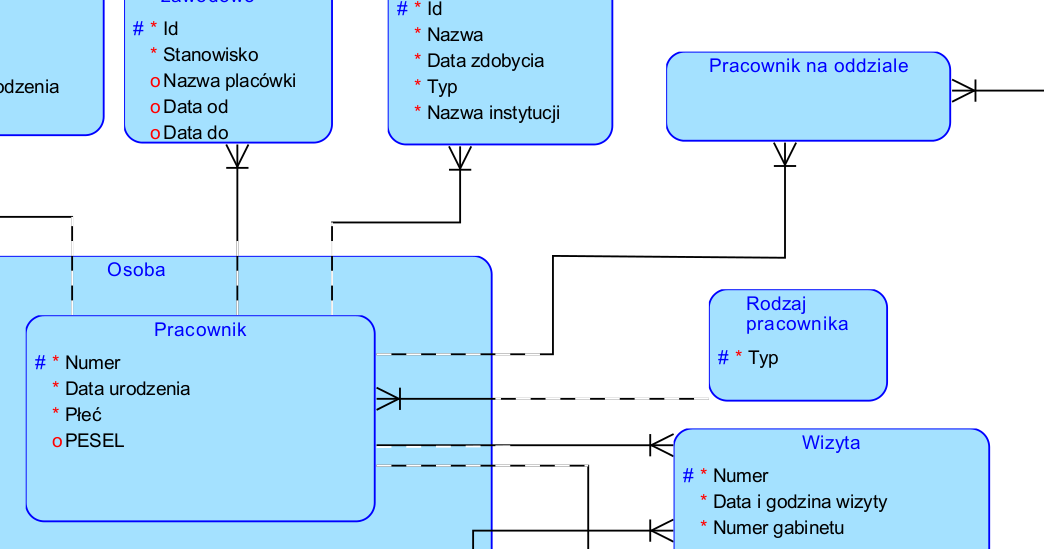
\includegraphics[width=0.7\textwidth]{img/p_n_o.png}
\caption{\small Nowa encja ,,Pracownik na oddziale''.}
\label{fig:pno}
\end{figure}

\clearpage

\textbf{Uzupełniono i uaktualniono tabele encji oraz ich atrybuty w sprawozdaniu dla fazy konceptualnej.} Dodano wszelkie encje spełniające funkcję encji słownikowych, czyli encje ,,Rodzaj umowy'', ,,Typ pokrewieństwa'', ,,Rodzaj pracownika", ,,Stan cywilny''. Określono dla nich unikalny identyfikator. Poniżej zaprezentowano reprezentację encji słownikowych w modelu ER.

\begin{figure}[H]
\centering
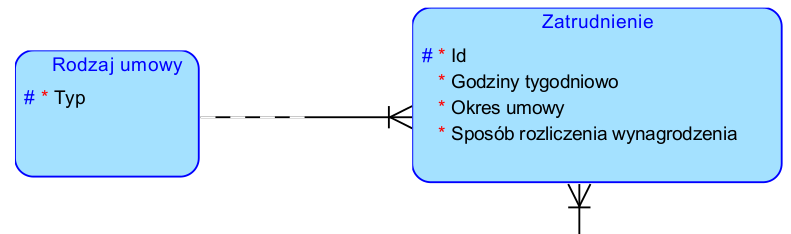
\includegraphics[width=0.7\textwidth]{img/rodzaj_umowy.png}
\caption{\small Encja ,,Rodzaj umowy''.}
\end{figure}

\begin{figure}[H]
\centering
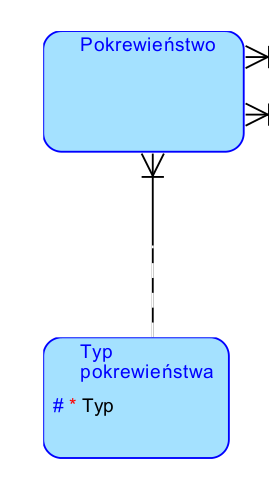
\includegraphics[width=0.25\textwidth]{img/typ_pokrewienstwa.png}
\caption{\small Encja ,,Typ pokrewieństwa''.}
\end{figure}

\begin{figure}[H]
\centering
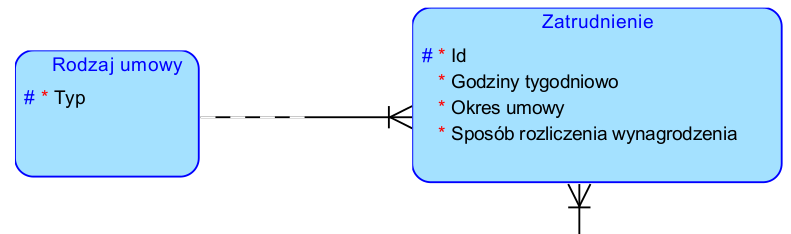
\includegraphics[width=0.7\textwidth]{img/rodzaj_umowy.png}
\caption{\small Encja ,,Rodzaj umowy''.}
\end{figure}

\begin{figure}[H]
\centering
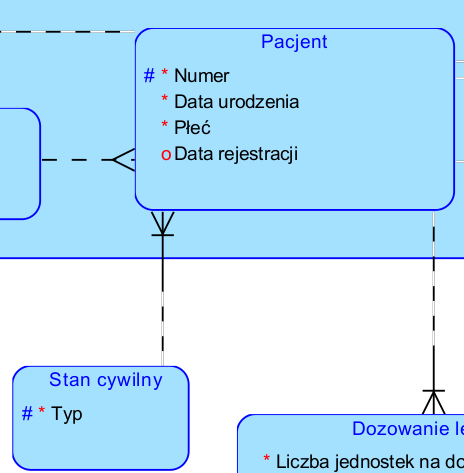
\includegraphics[width=0.4\textwidth]{img/stan_cywilny.png}
\caption{\small Encja ,,Stan cywilny''.}
\end{figure}



Uwzględniono również encję wiążącą encję główną ,,Osoba'' wraz z encją będąca jej podtypem ,,Pacjent". Jest to encja ,,Pokrewieństwo''.

\begin{figure}[H]
\centering
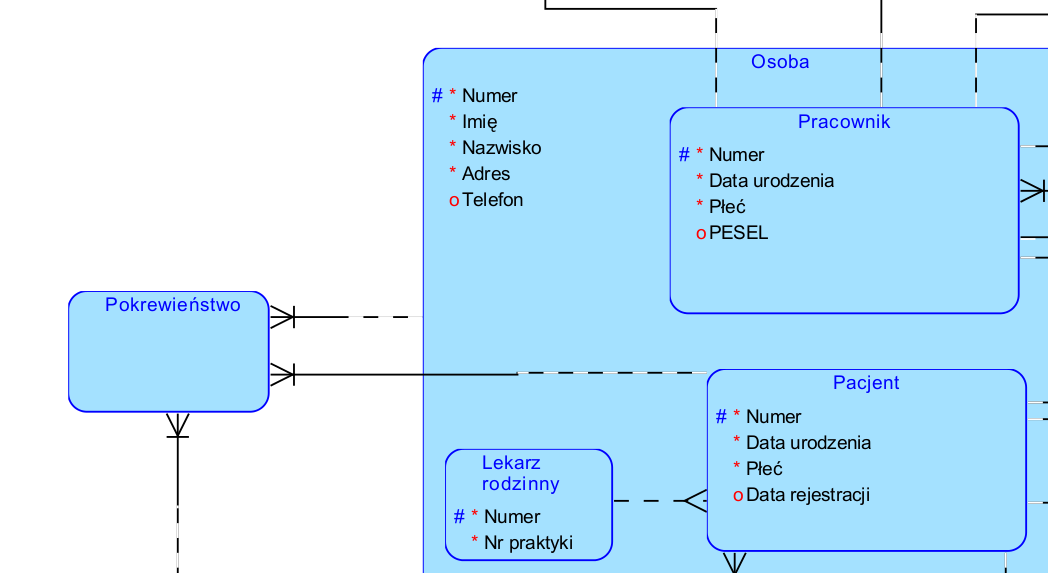
\includegraphics[width=0.7\textwidth]{img/pokrewienstwo.png}
\caption{\small Encja ,,Pokrewieństwo''.}
\end{figure}

\section{Niekompatybilności z modelem relacyjnym}
Pamiętając o przyszłej implementacji modelu relacyjnego w fizycznej bazie danych zwrócono uwagę, aby już na poziomie konceptualnym projektować związki i encje tak, aby dało się względnie łatwo i bez zbytniego narzutu przenieść projekt do logicznej postaci.

\textbf{Przy projektowaniu modelu nie wprowadzano związków ,,wiele-do-wielu''}. Zostały one zastępione dwoma związkami ,,jeden-do-wielu'' i nową encją pośrednią. 

Przykładem może być związek wielokrotny encji ,,Pacjent'' z encją ,,Oddział'', który został przekształcony na nową encję pomocniczą ,,Pracownik na oddziale'' oraz na dwa związki ,,jeden-do-wielu'' (Rysunek ~\ref{fig:pno}). Za pomocą ten encji wygenerowana zostanie relacja w modelu relacyjnym, która będzie składać się z dwóch kluczy obcych. Te dwa klucze obce utworzą klucz główny dla relacji.

Dla encji składających się z podtypów została wybrana częściowa \textbf{reprezentacja hybrydowa} w modelu relacyjnym ze względu na małą rendundancję danych i zmniejszenie potrzeby przechowywania tych samych informacji w różnych tabelach lub tworzenia dodatkowych widoków i więzów na tabele. Nie jest to najszybsze możliwe rozwiązanie, lecz pozwala uniknąć wielu błędów i niespójności w działaniu bazy. Stąd każdy podtyp dla encji ,,Osoba'', czyli encje ,,Pacjent'', ,,Pracownik'' oraz ,,Lekarz rodzinny'' będzie w modelu reacyjnym posiadał pojedynczy atrybut będący jednocześnie kluczem głównym oraz obcym (pochodzącym od relacji wygenerowanej z encji nadrzędnej). Jest to zilustrowanie na diagramie dla relacji ,,Pacjenci'', ,,Pracownicy'', ,,Lekarze rodzinni''.

\begin{figure}[H]
\centering
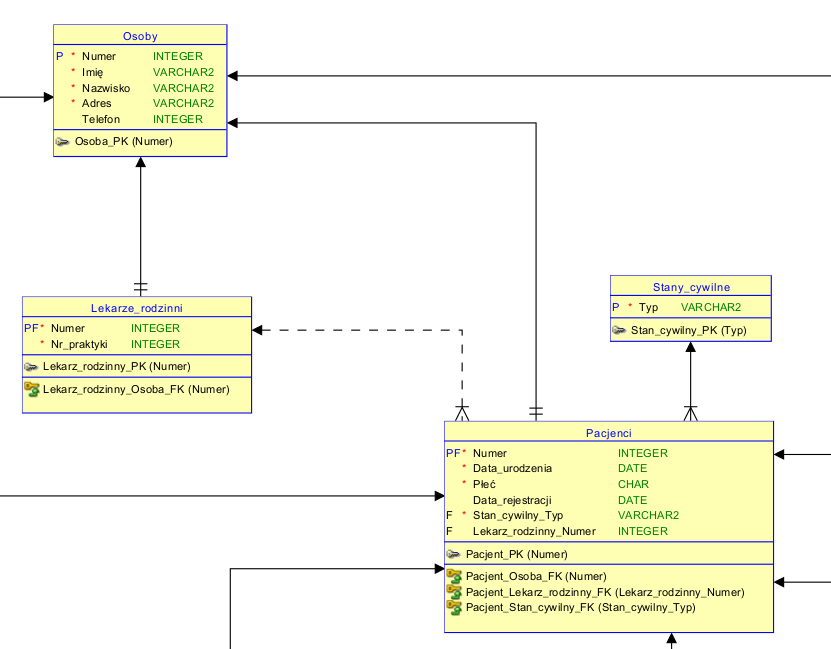
\includegraphics[width=0.7\textwidth]{img/podrzedne.png}
\caption{\small Zilustrowanie częściowej implementacji hybrydowej dla relacji ,,Osoby'', ,,Lekarze\_rodzinni,, oraz ,,Pacjenci''.}
\end{figure}

\clearpage

\textbf{Związki złożone od razu były zapisane przy pomocy dodatkowej encji posiadającej atrybut charakteryzujący wcześniejszy związek.} Przykładem takiego rozwiązania jest połączenie dwóch osób sprecyzowanym dla nich pokrewieństwem. Może istnieć sytuacja, w której pacjent będzie spokrewniony z osobą mającą związek ze szpitalem. Tym celu powstała encja ,,Pokrewieństwo''. W modelu relacyjnym jest ona reprezentowana jako relacja ,,Pokrewieństwa'', która posiada dwa klucze obce od relacji ,,Osoby'' oraz ,,Pacjenci'' i jeden atrybut charakteryzujący relację między nimi. Klucz prywatny ma zatem trzy segmenty na wszystkich atrybutach. Kluczem głównym jest atrybut mający właściwosć klucza obcego pochodzącego od relacji ,,Typy Pokrewieństwa''.

\begin{figure}[H]
\centering
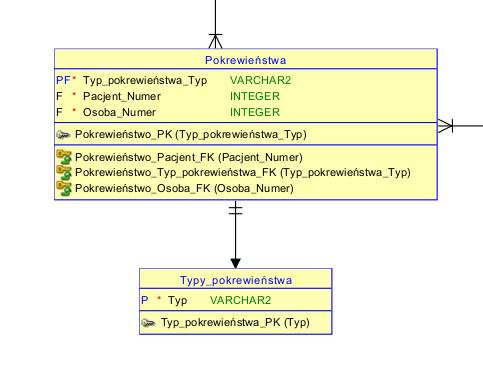
\includegraphics[width=0.5\textwidth]{img/pokrewienstwa.png}
\caption{\small Relacja ,,Pokrewieństwa''.}
\end{figure}

Relacja ,,Pokrewieństwa'' jest również jedną z kilku relacji, na których zastosowano zamianę atrybutu wielowartościowego na klucz obcy osobnej encji wyliczeniowej. Relacja ,,Typy pokrewieństwa'' posiada jeden atrybut będący kluczem głównym umieszczanym jako klucz obcy w encji ,,Pokrewieństwa'' zamiast atrybutu wieloznacznego. Innymi przykładami takiego zabiegu są relacje ,,Rodzaje pracowników'', ,,Stany cywilne'' oraz ,,Rodzaje umowy''.

\begin{figure}[H]
\centering
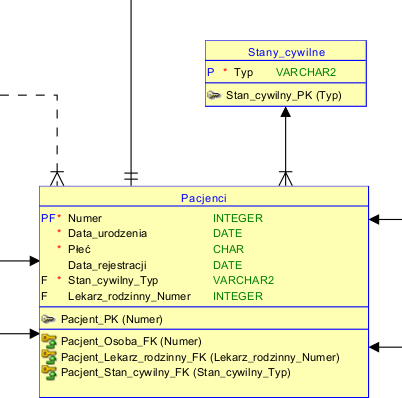
\includegraphics[width=0.5\textwidth]{img/stany_cywilne.png}
\caption{\small Relacja ,,Stany\_cywilne'' wraz z relacją ,,Pacjenci''.}
\end{figure}


\section{Wyznaczenie relacji}
% coś o kluczach
Wyznaczono relacje dla lokalnego logicznego modelu danych. Określono klucze główne oraz obce dla wszystkich relacji w modelu.

Wybrano odpowiednią reprezentację w modelu relacyjnym dla podtypów encji ,,Osoba'' - zastosowano częściową reprezentację hybrydową.

Ustandaryzowano nazewnictwo relacji w całym modelu. Relacje są nazwane reczownikami w liczbie mnogiej. Jeżeli istnieje więcej niż jeden człon dla nazwy relacji, to człony są odseparowane znakiem ,,\_''.


% coś o nazwach

\section{Normalizacja relacji}
Mając na względzie przyszłe aspekty normalizacji, zostały one uwzględnione już w fazie konceptualnej przy projektowaniu związków encji. 

Zwrócono szczególną uwagę, aby żadne informacje nie były nadmiarowe, aby nie były te same dane przechowywane w dwóch relacjach na raz. To utrudniałoby zachowanie poprawności danych przy modyfikacji.
% coś więcej 

\section{Weryfikacja transakcji przez model logiczny}
% czy działa
W ramach projektu sprawdzono, czy otrzymany model logiczny umożliwia realizację przykładowych transakcji opisanych poniżej.
% TODO

\begin{enumerate}


\item Utworzenie, aktualizowanie, wyszukiwanie informacji o pracownikach.

Dodajemy Osobę, Rodzaj\_pracownika (jeśli jeszcze taki nie istnieje) i Pracownika łącząc odpowiedznie klucze obce.

\item Wyszukiwanie pracowników o konkretnych kwalifikacjach bądź doświadczeniu zawodowym.

W zależności od wymaganych informacji przechodzimy po tabeli Pracownicy lub łączymy ją razem z osobami.

\item Pobranie listy pracowników ze szczegółowymi danymi dla danego oddziału.

Łączymy abele Oddziały, Pracownicy\_na\_oddziale i Pracownicy.

\item Tworzenie i przechowywanie szczegółowych informacji o pacjentach  skierowanych do szpitala.

Jeżeli nie ma wolnego miejsca na przyjęcie Pacjenta, to dodajemy wiersz do tabeli Pacjenci\_oczekujący. W przeciwnym przypadku dodajemy wiersz do tabeli Hospitalizacja.

\item Tworzenie i przechowywanie szczegółowych informacji o pacjentach ambulatoryjnych.

Tak jak wyżej, przy czym dodajemy wiersz również do tabeli Hospitalizacja\_ambulatoryjna.

\item Utworzenie raportu o pacjentach hospitalizowanych w danych oddziale.

Łączymy cztery tabele --- Oddziały, Łóżka, Hospitalizacje i Pacjenci.

\item Utworzenie raportu z informacjami o pacjentach oczekujących na przyjęcie na dany oddział.

Łączymy trzy tabele --- Oddziały, Pacjent\_oczekujący i Pacjenci.

\item Tworzenie, aktualizacja i pobieranie informacji o lekarstwach podawanych danemu pacjentowi.

Łączymy tabele Dozowania\_leku, Leki, Materiały i Pacjenci.

\item Pobranie informacji o lekarstwach, które należy podać oraz o której godzinie pacjentom w danym dniu.

Łączymy Dozowania\_leku, Leki i Pacjenci. Obliczamy godzinę podania. Dla wygody pielęgniarek można także dodać informację o Łóżku, na którym leży Pacjent.

\item Tworzenie i  modyfikowanie informacji o dostawcach, z którymi współpracuje szpital.

Zwracamy lub modyfikujemy dane z tabeli Dostawcy nie łącząc z żadną inną.

\item Pobranie informacji o wszystkich materiałach dostarczonych danemu oddziałowi w wybranym zakresie dat.

Wszystkie Formularze\_zapotrzebowania z niezerową datą otrzymania w określonym przedziale i z określonym Oddziałem. Łączymy to z pozycjami formularza i Materiałami.

\item Sprawdzenie, edytowanie warunków zatrudnienia danego pracownika szpitala.

Zwracamy i modyfikujemy tabelę Zatrudnienia dla danego Pracownika.

\item Przeglądanie listy wizyt przypisanych danemu pracownikowi szpitala.

Wypisujemy wszystkie Wizyty dla danego Pracownika i łączymy z Pacjentami.

\item Wyszukanie przez pacjenta przypisanej mu wizyty.

Wypisujemy wszystkie Wizyty dla danego Pacjenta.

\item Utworzenie raportu z aktualnym stanem zajmowanych łóżek przez pacjentów na danym oddziale.

Wyszukujemy wszystkie obecnie trające Hospitalizacje, czyli te, których Faktyczna\_data\_wypisania jest nieokreślona. Łączymy to z Łóżkami i danym Oddziałem.

\end{enumerate}

\section{Wyznaczenie więzów integralności}
% kiedy atrybut jest wymagany
% czy są jakieś atrybuty unikalne nie będące kluczami
Dla stworzonego modelu relacyjnego wprowadzono więzy integralności, które pozwalają na utrzymanie spójności bazy danych. W ramach utrzymania integralności encji, wszystkie tabele mają swój własny klucz główny (\textit{PRIMARY KEY}). W zależności od tabeli na klucz główny może się składać kilka atrybutów (kolumn).

\begin{figure}[H]
\centering
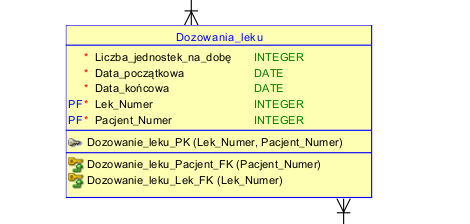
\includegraphics[width=0.55\textwidth]{img/dwa_PK.png}
\caption{\small Przykład złożonego klucza głównego.}
\end{figure}

Dla tabel wyznaczono więzy na integralność krotek. Między innymi zawężono dziedziny atrybutów w szczególności dla atrybutów typu \textit{VARCHAR2}. W ten sposób usunięto nieporzebną nadmiarowość związaną z przechowywaniem wartości atrybutów. Określono również typ jednostki -\textit{BYTE} lub \textit{CHAR}. Dla atrybutów wprowadzono więzy na zawężenie dziedziny do liczby elementów typu \textit{CHAR} z racji uniezależnienia się od aktualnego formatu kodowania znaków w systemie (np. UTF-8) - wybranie reprezentacji \textit{BYTE} mogłoby spowodoać niekompatybilności związane z tym, że jeden znak (litera) może być zakodowania na więcej niż jednym bajcie. W przypadku atrybutu określającego adres email w tabelach zastosowano typ \textit{BYTE}.

\begin{figure}[H]
\centering
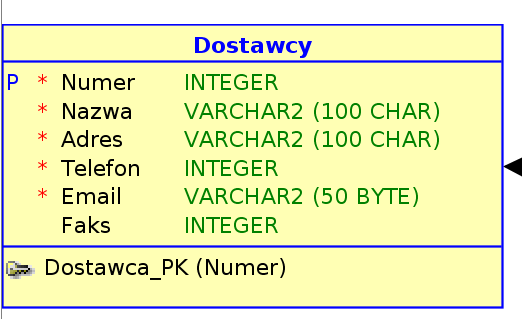
\includegraphics[width=0.5\textwidth]{img/dostawcy.png}
\caption{\small Przykład nałożenia więzów integralności dla krotek.}
\end{figure}

Dla relacji ,,Dostawy'' określono skalę i precyzję atrybutu typu NUMBER wyznaczającego koszt jednostkowy materiału w ramach jego dostawy do szpitala.

\begin{figure}[H]
\centering
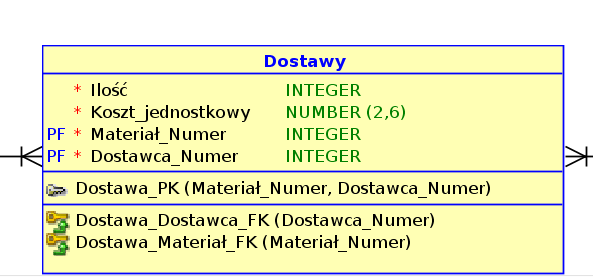
\includegraphics[width=0.7\textwidth]{img/dostawy.png}
\caption{\small Przykład nałożenia więzów integralności dla krotek dla atrybutu ,,Koszt\_jednostkowy'' .}
\end{figure}

\clearpage

Zadbano o odpowiednią integralność odwołań. W tym celu niektóre tabele posiadają klucze obce (\textit{FOREIGN KEY}). Poniżej przestawiono przykład tabeli ,,Zatrudnienia'' posiadającej dwa atrybuty będące kluczami obcymi. Odwołują się one do odpowiednich tabel ,,Rodzaje\_umowy'' oraz ,,Pracownicy''.

\begin{figure}[H]
\centering
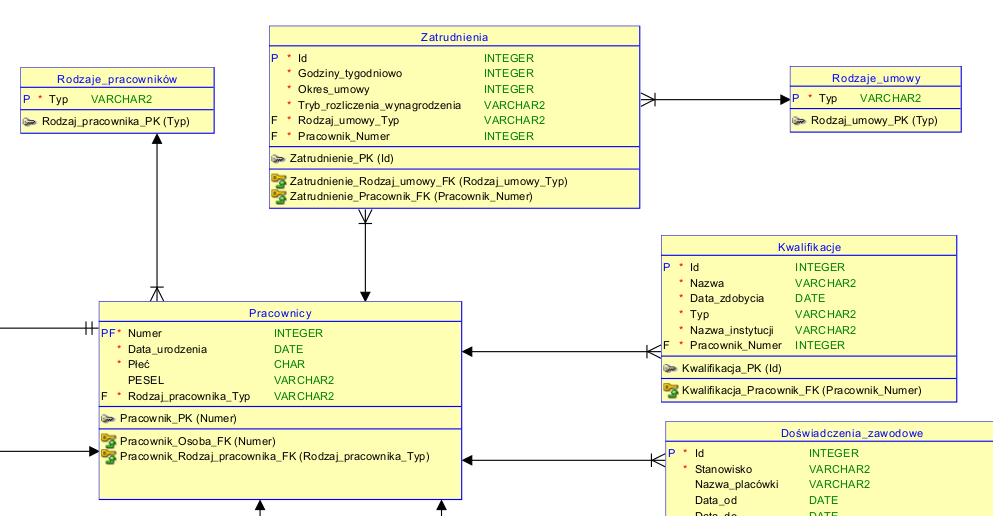
\includegraphics[width=0.85\textwidth]{img/itegralnosc_odwolan.png}
\caption{\small Przykład zastosowania kluczy obcych dla tabeli ,,Rodzaje\_umowy''.}
\end{figure}

Baza nie posiada innych więzów integralności, takich jak wymaganie wartości NULL na dokładnie jednym z dwóch atrybutów, poprawność numerów: telefonu, PESEL, NIP itp.

% todo - opisać to szerzej


\section{Wykres modelu logicznego}
% opowiedzieć i zamieścić diagram żółtych tabel
Wykres modelu logicznego załączono do sprawzodania w formacie \textit{PDF}.

\section{Uzupełnienie diagramu ER}
\textbf{Diagram został uzupełniony i poprawiony}, aby automatycznie mógł być przekonwertowany do diagramu logicznego. Niestety, otrzymany diagram logiczny wymagał jeszcze sporej ilości ręcznych poprawek takich jak usuwanie niepotrzebnych kluczy i więzów oraz zmiany nazw tabel i atrybutów.

Do diagramu związków encji dodano wspomniany wyżej związek wieloznaczny (zamieniony odpowiednio na encję i dwa związki) i ustanowiono odpowiednie do przechowywanych danych typy atrybutów.

\textbf{Wprowadzono specjalną encję nazwaną ,,Pracownik na oddziale''}. Umożliwia ona powiązanie encji ,,Pracownik'' z encją ,,Oddział''. W ten sposób możliwe będzie zrealizowanie transakcji na bazie danych polegającej na pobraniu listy pracowników ze szczegółowymi danymi dla danego oddziału.

W ramach uzupełnienia diagramu ER \textbf{dodano do niektórych encji (przede wszystkim encji słownikowych) unikalne identyfikatory}.
Dla encji będących podtypami encji ,,Osoba'', czyli ,,Pracownik'', ,,Pacjent'' oraz ,,Lekarz rodzinny'' dodano jako dodatkowy atrybut nazwany ,,Numer''. Spełnia rolę on unikalnego identyfikatora dla każdej z tych encji. Dzięki temu będzie możliwy efektywniejszy dostęp do danych pracowników i pacjentów szpitala. Dodanie unikalnego identyfikatora oraz atrybutu ,,Numer'' wykonano dla  również dla encji ,,Pozycja zamówienia'', ,,Formularz zamówienia'' oraz ,,Hospitalizacja''.



\end{document}